% latex foo.tex 
% dvips -Poutline -G0 foo.dvi -o 
% ps2pdf -dPDFSETTINGS#/prepress foo.ps
\documentclass[slidestop,xcolor=pst,dvips]{beamer}
\usepackage{fancyvrb}
\usepackage{hyperref}
\usepackage{pstricks,pst-tree,pst-node,pst-plot}
\usepackage{graphicx}


\newcommand{\sect}[1]{
\section{#1}
\begin{frame}[fragile]\frametitle{#1}
}

\newcommand{\myvec}[1]{
\pstThreeDDot[showpoints=true,drawCoor=true](#1)
\pstThreeDLine[arrows=->,linecolor=blue](0,0,0)(#1)
}


\mode<presentation>
{
  \usetheme{Madrid}
  % or ...

%  \setbeamercovered{transparent}
  % or whatever (possibly just delete it)
}

\usepackage[english]{babel}

\usepackage[latin1]{inputenc}

\title[Computer Graphics, CSCI 480]
{
Noise
}

\subtitle{} % (optional)

\author[Geoffrey Matthews]
{Geoffrey Matthews}
% - Use the \inst{?} command only if the authors have different
%   affiliation.

\institute[WWU/CS]
{
  Department of Computer Science\\
  Western Washington University
}
% - Use the \inst command only if there are several affiliations.
% - Keep it simple, no one is interested in your street address.

\date{Fall 2012}

% If you have a file called "university-logo-filename.xxx", where xxx
% is a graphic format that can be processed by latex or pdflatex,
% resp., then you can add a logo as follows:

\pgfdeclareimage[height=0.5cm]{university-logo}{WWULogoProColor}
\logo{\pgfuseimage{university-logo}}

% If you wish to uncover everything in a step-wise fashion, uncomment
% the following command: 

%\beamerdefaultoverlayspecification{<+->}

\begin{document}

\psset{arrowscale=2}

\begin{frame}
  \titlepage
\end{frame}


\newcommand{\myref}[1]{\small\item\url{#1}}
\newcommand{\myreft}[1]{\footnotesize\item\url{#1}}

%\begin{frame}
%  \frametitle{Outline}
%  \tableofcontents
%  % You might wish to add the option [pausesections]
%\end{frame}

\sect{Noise}
\begin{columns}[T]
\column{0.75\textwidth}
\begin{itemize}
\item Idea is to define a function that looks like the randomness we
  find in nature.
\item Dirt, clouds, waves on the ocean, skin, all exhibit randomness.
\item However, it is not {\bf white noise}, seen at upper right.
It is much smoother, as seen at lower right.
\item Real world noise exhibits smoothness, going from dark to light
  gradually, with dark and light patches randomly distributed.
\item How can we simulate that?  We will add up smoothed white noise
  at different wavelengths, with the {\em
    amplitude} of the noise proportional to its {\em wavelength}.
\item This is called {\bf pink noise}.

\end{itemize}

\column{0.25\textwidth}
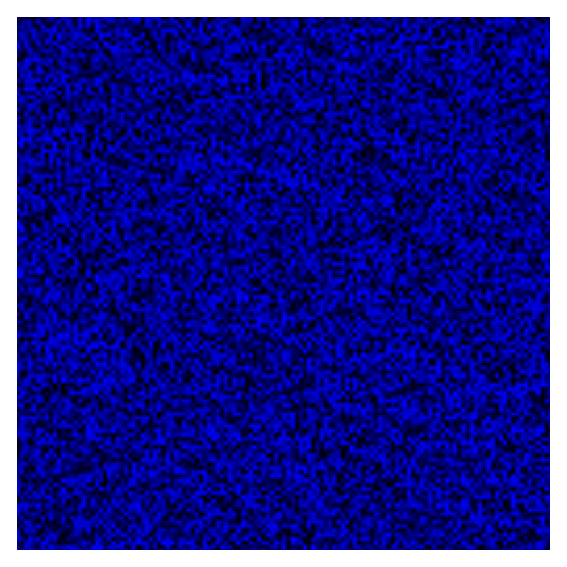
\includegraphics[width=\textwidth]{whitenoise.eps}
\vfill

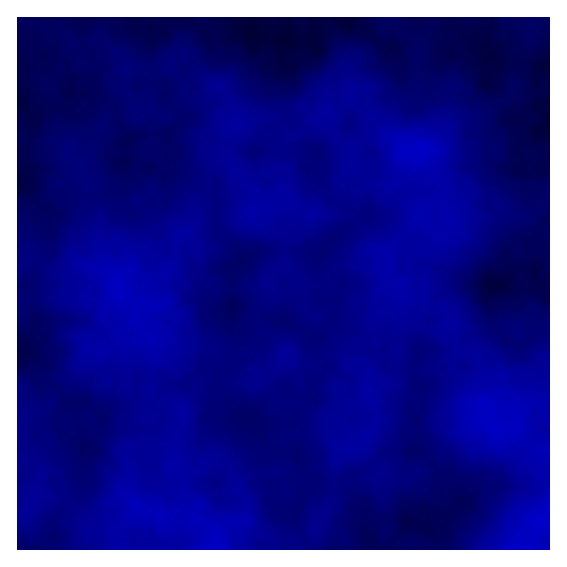
\includegraphics[width=\textwidth]{pinknoise.eps}
\end{columns}
\end{frame}

\sect{Adding up sin curves}
\centerline{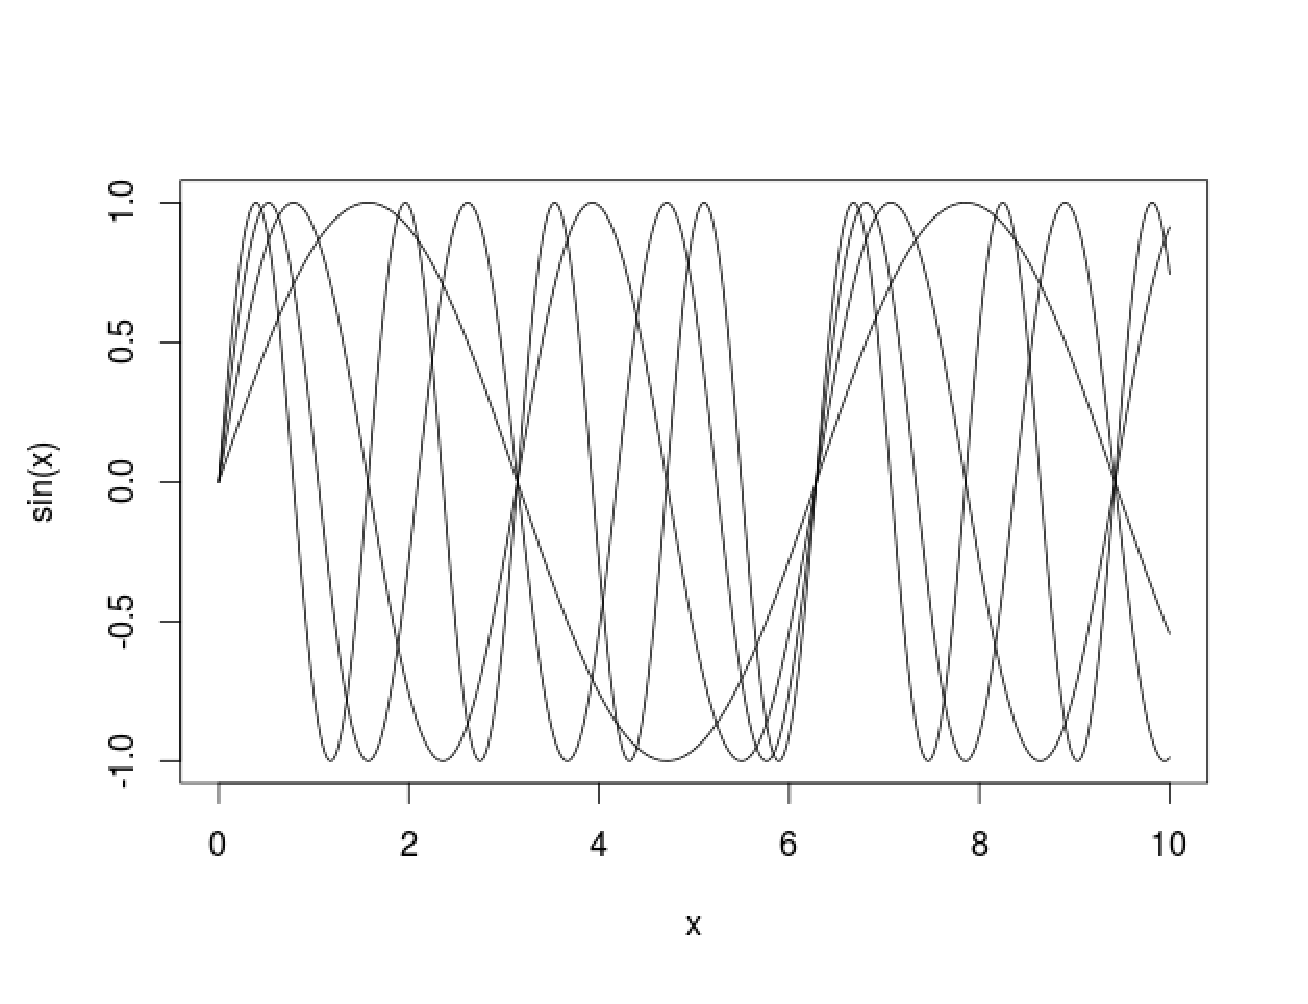
\includegraphics[width=4in]{figures/sincurves.eps}}
\end{frame}
\sect{Adding up sin curves}
\centerline{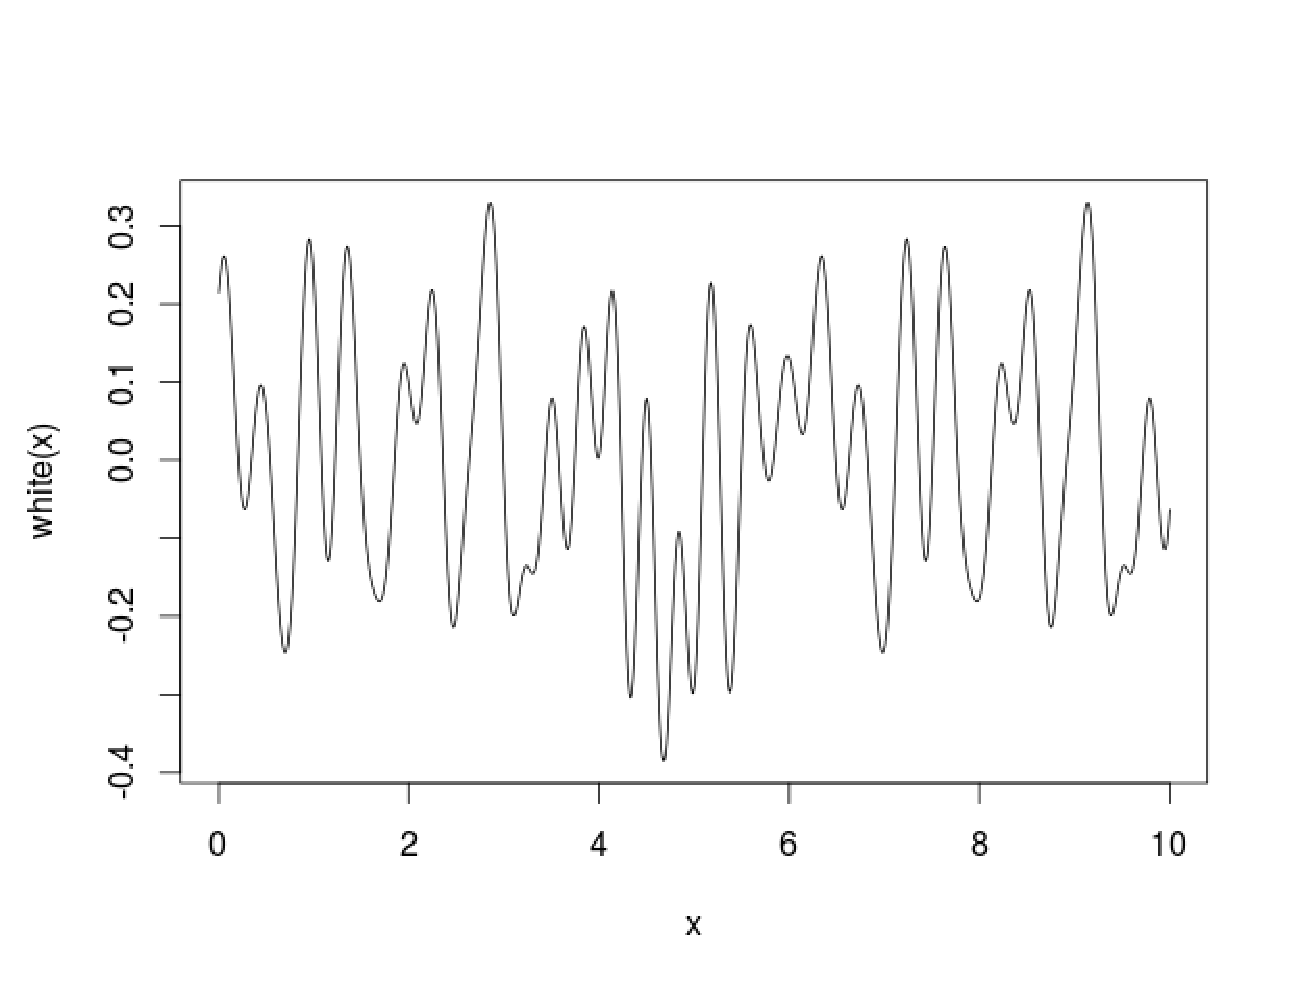
\includegraphics[width=4in]{figures/whitenoisecurves.eps}}
\end{frame}


\sect{Adding up scaled sin curves}
\centerline{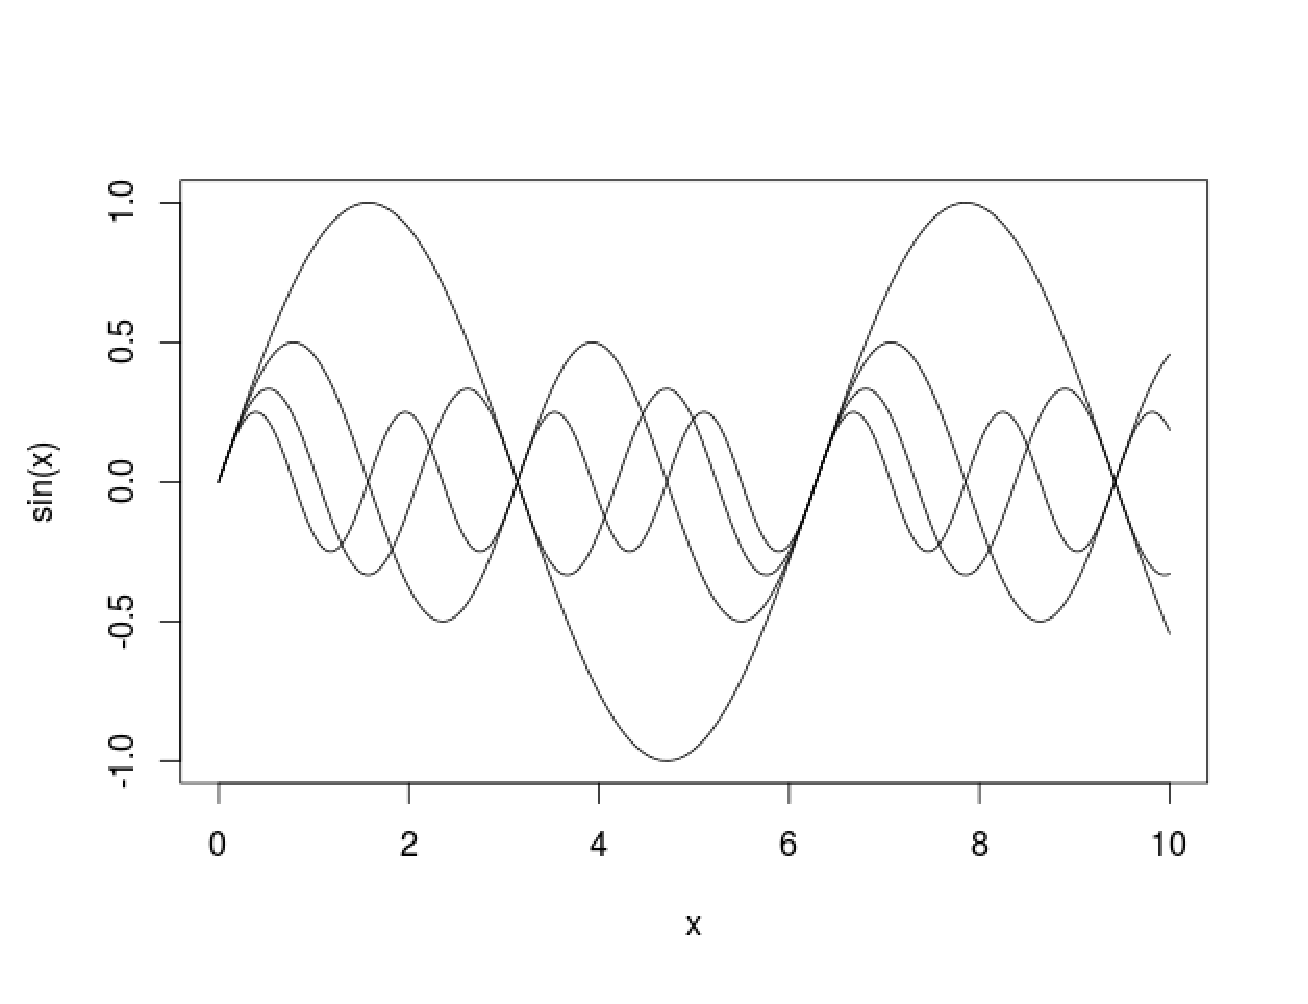
\includegraphics[width=4in]{figures/scaledsincurves.eps}}
\end{frame}
\sect{Adding up scaled sin curves}
\centerline{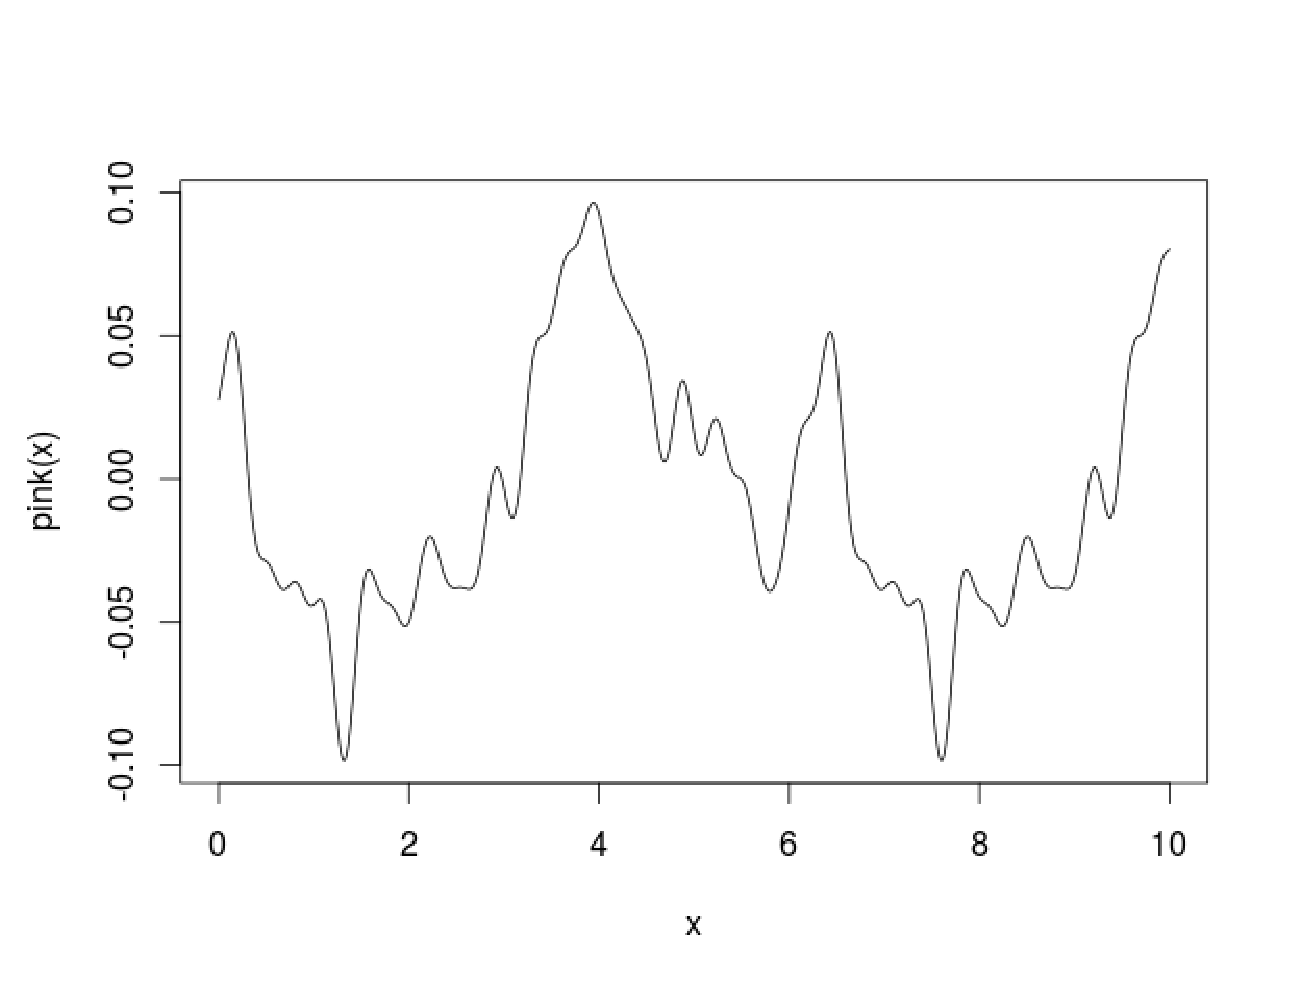
\includegraphics[width=4in]{figures/pinknoisecurves.eps}}
\end{frame}


\sect{Defining a lattice over screen space.}
\begin{pspicture}[showgrid=true](-1,-1.1)(10,5)
\psline(0,0)(6.4,0)(6.4,4.8)(0,4.8)(0,0)
\pcline[offset=-0.3]{|<->|}(0,0)(6.4,0)
\ncput*[nrot=:U]{640 pixels}
\pcline[offset=0.3]{|<->|}(0,0)(0,4.8)
\ncput*[nrot=:U]{480 pixels}
\uput[45](8,-1){Lattice coordinates}
\end{pspicture}
\begin{itemize}
\item Divide by the {\em wavelength}, the distance between lattice lines.
\item Optionally, flip the origin to lower left.
\end{itemize}
\end{frame}

\sect{latticeNoise: A white noise value for lattice points}

\includegraphics[width=\textwidth]{randompoints.eps}

\begin{itemize}
\item We start with just a single dimension, $x$ (scaled to lattice space).
\item \verb|latticeNoise| only defined at integers.
\item White noise values between 0 and 1
\item Our space is generally too big for an array for all those
  numbers, so we will find a function \verb+latticeNoise(x)+ that
  uses less memory but is still very fast.
\end{itemize}
\end{frame}

\sect{latticeNoise: a Simple Implementation}

\begin{itemize}
\item Pick a modest array size, normally $n=256$\\
   ... but for illustration we use $n = 8$
\item Create an array of $n$ floats evenly spaced between 0 and 1, {\em e.g.},\\
\verb|noiseTable = (0.00,0.14,0.29,0.43,0.57,0.71,0.86,1.00)|
\item We could randomize this table, but instead we randomize the
  index into this table. We use a permutation of the first $n$ integers, {\em e.g.},\\
  \verb|hashTable = (5,2,7,1,0,3,4,6)|
\item Our function becomes\\ 
\verb|latticeNoise(x): return noiseTable[hashTable[x%n]]|,
\item This will be very fast.
\item {\em Note: The sequence repeats every $n$ integers, but that won't be as
  important when we move up to 2 and 3 dimensions.}
\pause\item Do {\tt noiseTable} and {\tt hashTable} have to be the same size?
\end{itemize}
\end{frame}

\sect{latticeNoise: A white noise value for lattice points}

\includegraphics[width=\textwidth]{randompoints.eps}

\begin{itemize}
\item  \verb|hashTable = (5,2,7,1,0,3,4,6)|
\item \verb|noiseTable = (0.00,0.14,0.29,0.43,0.57,0.71,0.86,1.00)|
\item \verb|latticeNoise(x): return noiseTable[hashTable[x%n]]|
\end{itemize}
\end{frame}


\sect{lerpNoise: filling in between the lattice points}

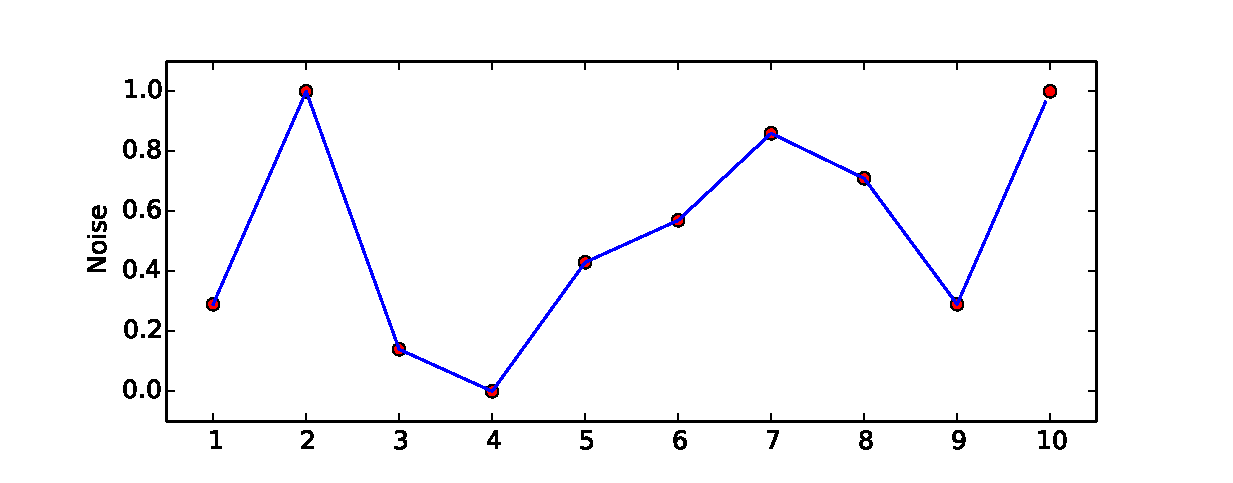
\includegraphics[width=\textwidth]{randomlerped.eps}

\begin{itemize}
\item One option is to use linear interpolation.
\item Better than white noise.
\item Easy to compute:  \verb|lerp(pct, a, b): a + pct*(b-a)|
\item However, makes for a spikey curve, not like the noise we find in nature.
\end{itemize}


\end{frame}

\sect{smerpNoise: Smoothly Interpolate Between the Integers}
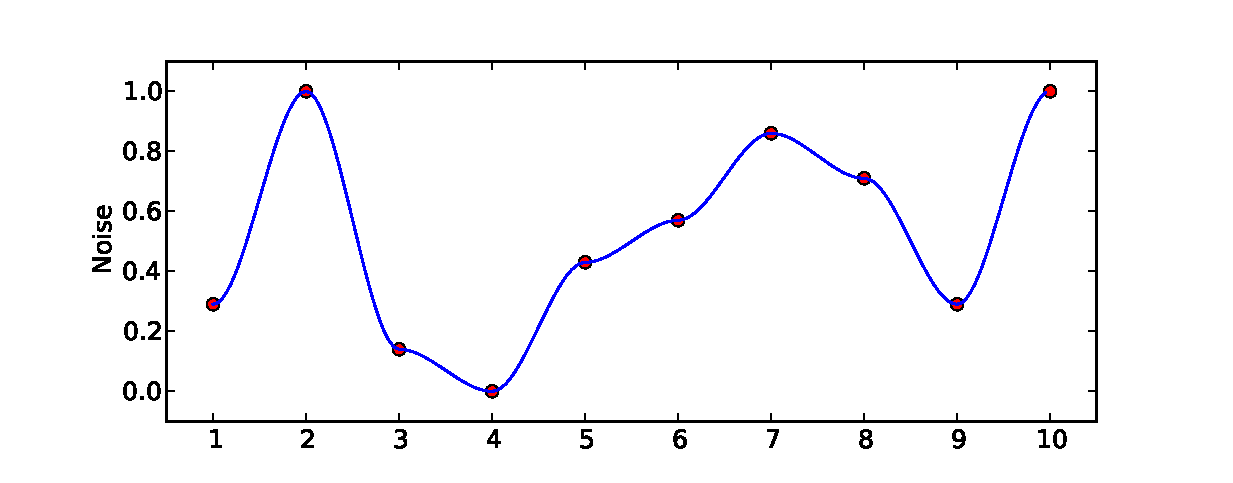
\includegraphics[width=\textwidth]{randomsmoothed.eps}

\begin{itemize}
\item This looks more like what we want.
\item There are many ways to compute smooth curves through a set of
  points.
  Look up {\bf
    B-splines}, {\bf Hermite curves}, and {\bf Bezier curves}.
\item  Here we want a simpler approach: an easily computable 
  {\bf S-curve} between each pair of points.
\end{itemize}
\end{frame}


\sect{S-curve}
\centerline{\includegraphics[width=0.6\textwidth]{scurve.eps}}

\begin{itemize}
\item There are many S-curves, such as the {\bf logistic function}, or
  even the {\bf cosine} function between 0 and $\pi$, but we can come
  up with our own easily enough.  It would help if we could avoid
  transcendental functions, too.  (Why?)
\item The S-curve we need smoothly maps the 0-1 interval to
itself, and is horizontal at
  both ends.
\item What might be a good approach?
\end{itemize}
\end{frame}

\sect{S-curve}
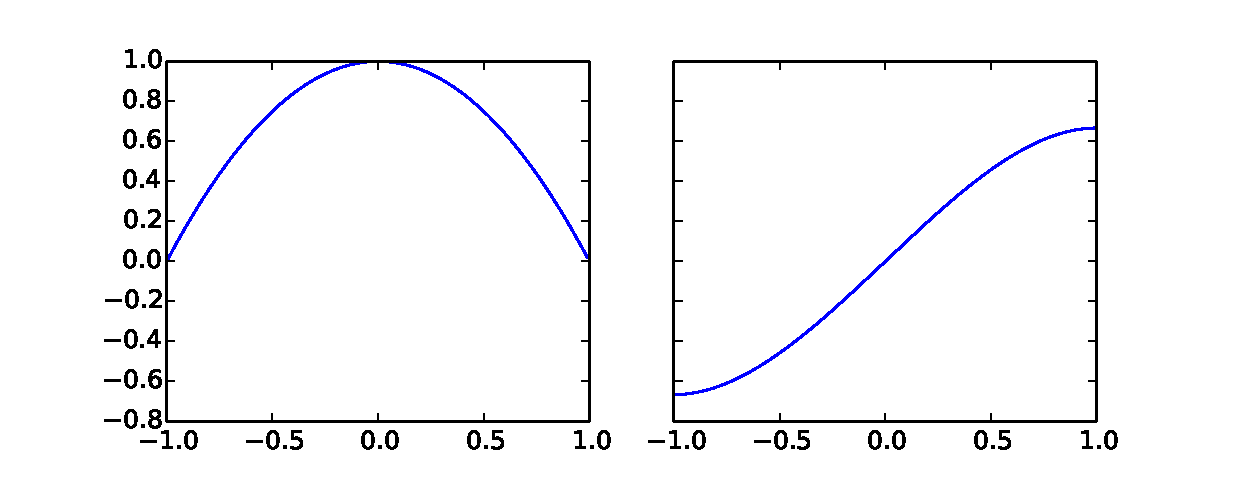
\includegraphics[width=\textwidth]{cubescurve.eps}

\begin{itemize}
\item On the left we plot $1-x^2$.  This is zero at $\pm1$, which
  means any curve that has this as its derivative will be horizontal
  at $\pm1$
\item On the right we plot $x - \frac{x^3}{3}$.  Shifting and scaling leads to:
\begin{verbatim}
smerp(pct, a, b):
    x = ???
    return a + (??? + ???*x - ???*x*x*x)*(b-a)
\end{verbatim}

\end{itemize}

\end{frame}

\sect{smerpNoise: Smoothly Interpolate Between the Integers}
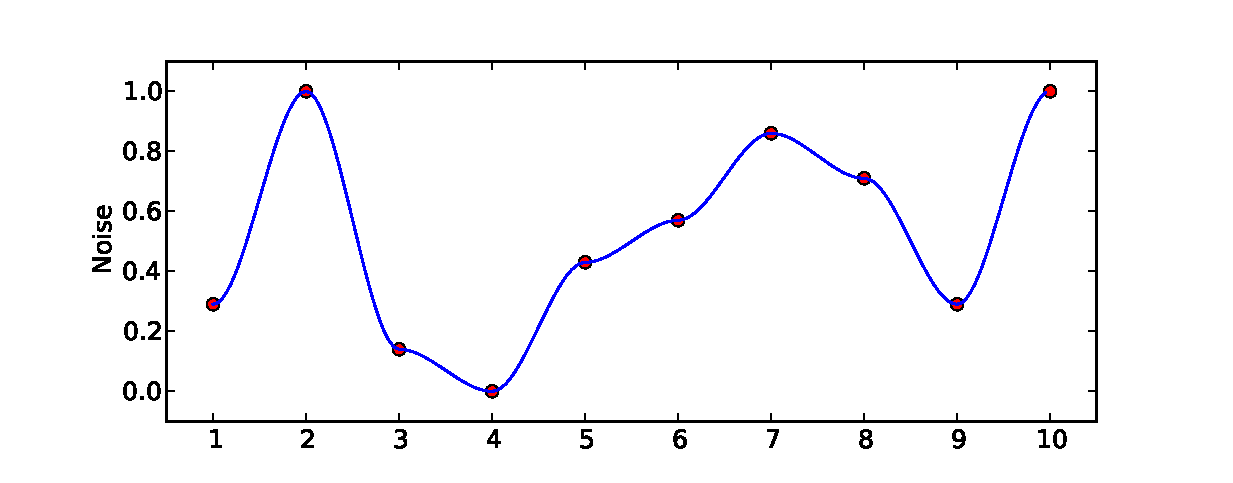
\includegraphics[width=\textwidth]{randomsmoothed.eps}

\begin{itemize}
\item The curve height is always between 0 and 1.
\item The derivative of the curve is zero at lattice points.
\item Highest and lowest points will always be at lattice points.
\item Repeats after $n$ lattice points.
\item We would like the curve to have more detail at smaller scales, so
  we move on to {\em pink noise}. 
\end{itemize}

\end{frame}

\sect{Pink Noise}
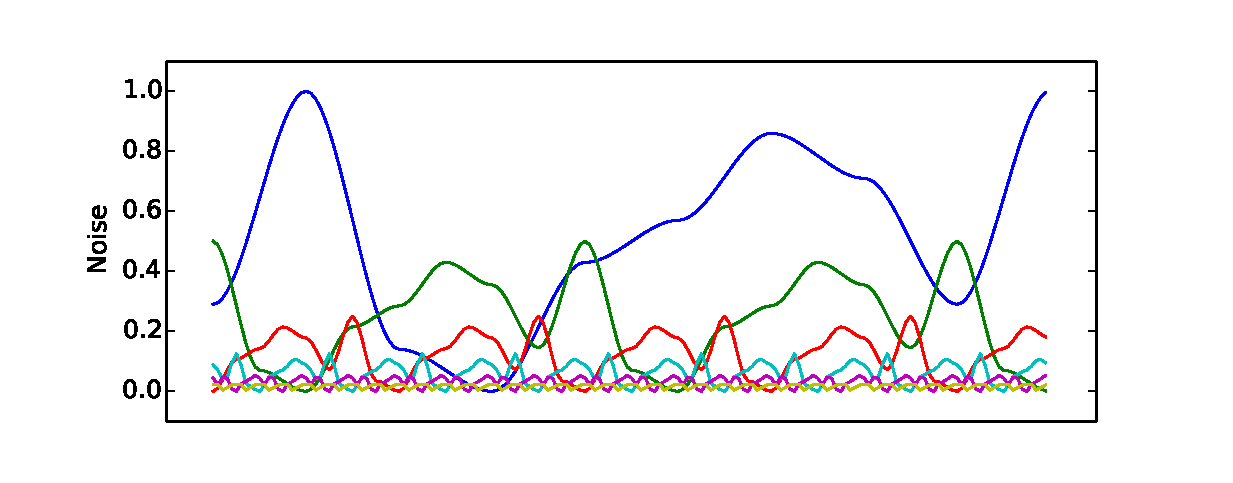
\includegraphics[width=\textwidth]{pinkseparate.eps}

\begin{itemize}
\item Lattice distance is arbitrary, so we can scale the lattice frequency.
\item We can also scale the maximum amplitude.
\item Here we show curves for $i$ from 0 to 5:
\begin{itemize}
\item \verb|smerpNoise(x*2**i)/2**i|
\end{itemize}
\item Amplitude has a $1/f$ relationship to frequency.
\end{itemize}

\end{frame}

\sect{Pink Noise}
\includegraphics[width=\textwidth]{pinksummed.eps}

\begin{itemize}
\item Here we show the sum for $i$ from 0 to 5 of:

 \verb|smerpNoise(x*2**i)/2**i|

\item Sum is divided by 2.  Why?
\item This is also an example of {\bf fractal Brownian motion } (fBm).
\end{itemize}
\end{frame}

\sect{Pink Noise}
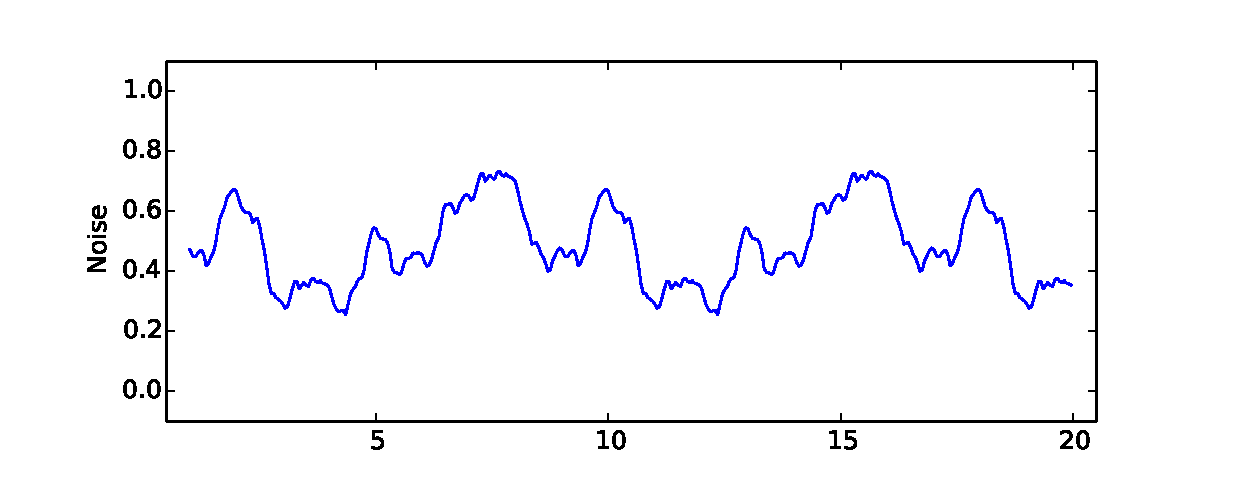
\includegraphics[width=\textwidth]{pinksummedlargerange.eps}

\begin{itemize}
\item If we look at a larger range, we can see that it still repeats
  after $n$ integers.  Why?
\item Could we fix that?  How?
\end{itemize}
\end{frame}

\sect{Pink Noise without repeats}

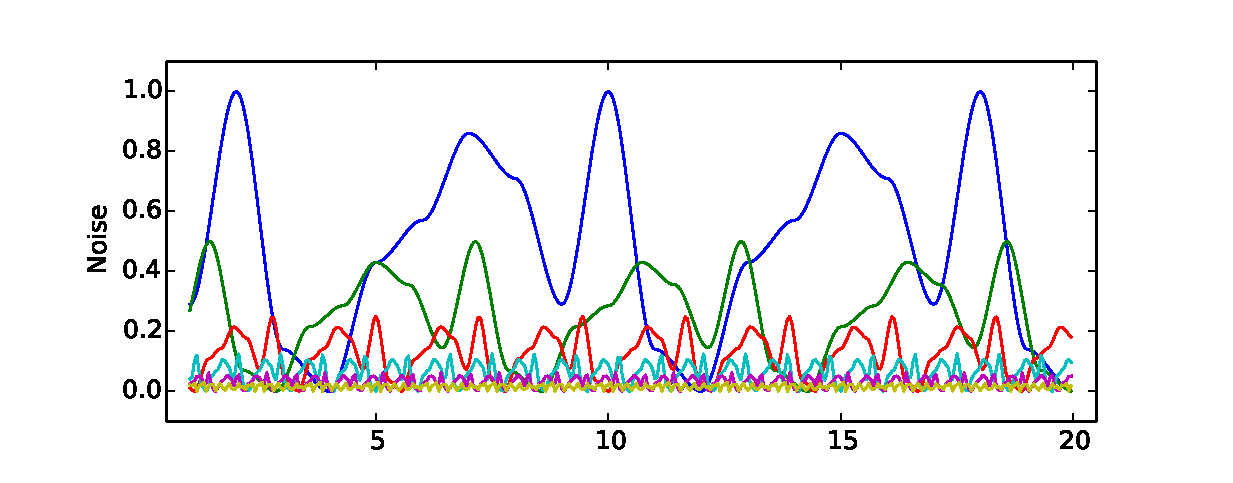
\includegraphics[width=\textwidth]{pinknoiseprime.eps}

\begin{itemize}
\item We rescale each wavelength by a small amount, so they don't line up.
\end{itemize}
\end{frame}

\sect{Pink Noise without repeats}

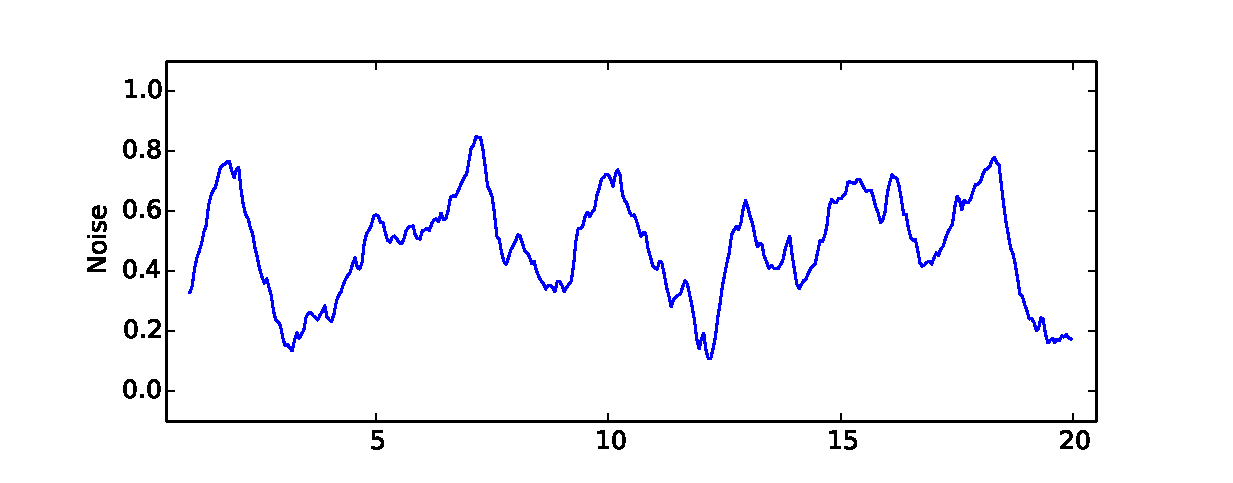
\includegraphics[width=\textwidth]{pinknoiseprimesummed.eps}

\begin{itemize}
\item When we add them up they don't repeat for a long time.
\item This would be even more effective with a larger $n$, {\em e.g.}
  256.
\item However, we won't do this because the problem will be solve itself
  in higher dimensions.
\end{itemize}
\end{frame}

\sect{Lattice Noise in 2D}

\psset{unit=1.5}
\begin{pspicture}(-1,-0.25)(3.5,2.5)
\psaxes[]{->}(0,0)(4,2.5)
\rput(1,1){\circlenode{A}{\tiny 0.14}}
\rput(2,1){\circlenode{A}{\tiny 0.88}}
\rput(3,1){\circlenode{A}{\tiny 0.21}}

\rput(1,2){\circlenode{A}{\tiny 0.19}}
\rput(2,2){\circlenode{A}{\tiny 0.51}}
\rput(3,2){\circlenode{A}{\tiny 0.23}}

\end{pspicture}

\begin{itemize}
\item For lattice noise in 2D we could use a two dimensional array of noise
  values, and a hashed lookup into that table:
\begin{verbatim}
    latticeNoise(x,y):
        noiseTable[hashTable[x%n], hashTable[y%n]]
\end{verbatim}
\item ... but there's a better way.
\end{itemize}
\end{frame}

\sect{Lattice Noise in 2D}

\psset{unit=1.5}
\begin{pspicture}(-1,-0.25)(3.5,2.5)
\psaxes[]{->}(0,0)(4,2.5)
\rput(1,1){\circlenode{A}{\tiny 0.14}}
\rput(2,1){\circlenode{A}{\tiny 0.88}}
\rput(3,1){\circlenode{A}{\tiny 0.21}}

\rput(1,2){\circlenode{A}{\tiny 0.19}}
\rput(2,2){\circlenode{A}{\tiny 0.51}}
\rput(3,2){\circlenode{A}{\tiny 0.23}}
\end{pspicture}

\begin{itemize}
\item We hash both $x$ and $y$ to get a single lookup into
  the same one-dimensional noise table:
\begin{verbatim}
    latticeNoise(x,y):
        noiseTable[hashTable[(x + hashTable[y%n])%n]]
\end{verbatim}
\item This solves the repetition problem, too.  Why?
\item What would we do in 3D?  4D?
\end{itemize}
\end{frame}

\sect{Smooth Noise in 2D}
\begin{columns}[T]
\column{0.65\textwidth}
\begin{itemize}
\item Now that we have our random values at the corners, we need to
  smoothly interpolate the ones in between:
\begin{verbatim}
smerpNoise2(x, y):
    intx = floor(x)
    inty = floor(y)
    pctx = x - intx
    pcty = y - inty
    aa = latticeNoise2(intx, inty)
    ab = latticeNoise2(intx, inty+1)
    ba = latticeNoise2(intx+1, inty)
    bb = latticeNoise2(intx+1, inty+1)
    xa = smerp(pctx, aa, ba)
    xb = smerp(pctx, ab, bb)
    return smerp(pcty, xa, xb)
\end{verbatim}
\end{itemize}
\column{0.35\textwidth}
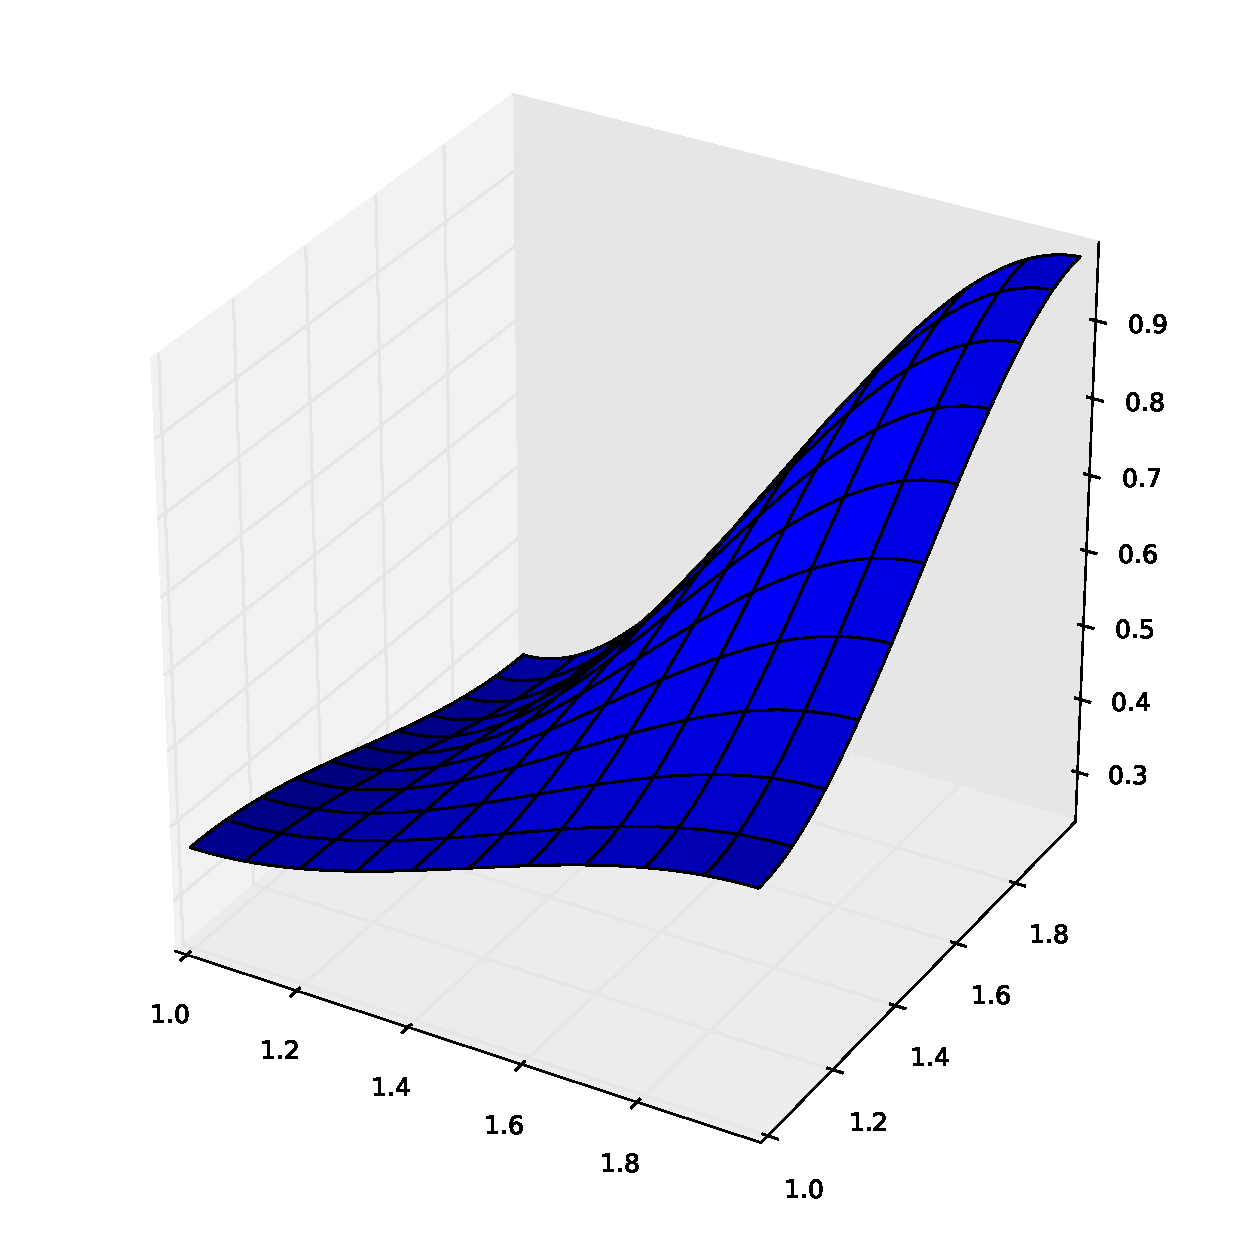
\includegraphics[width=\textwidth]{onesquaresurface.eps}
\end{columns}
\end{frame}


\sect{Smooth Noise in 2D}
\begin{columns}[T]
\column{0.5\textwidth}
\begin{itemize}
\item What does the interpolation function look like in 3D?
\item  4D?
\item Do you see a problem?
\item Look up {\bf simplex noise}.
\end{itemize}
\column{0.5\textwidth}
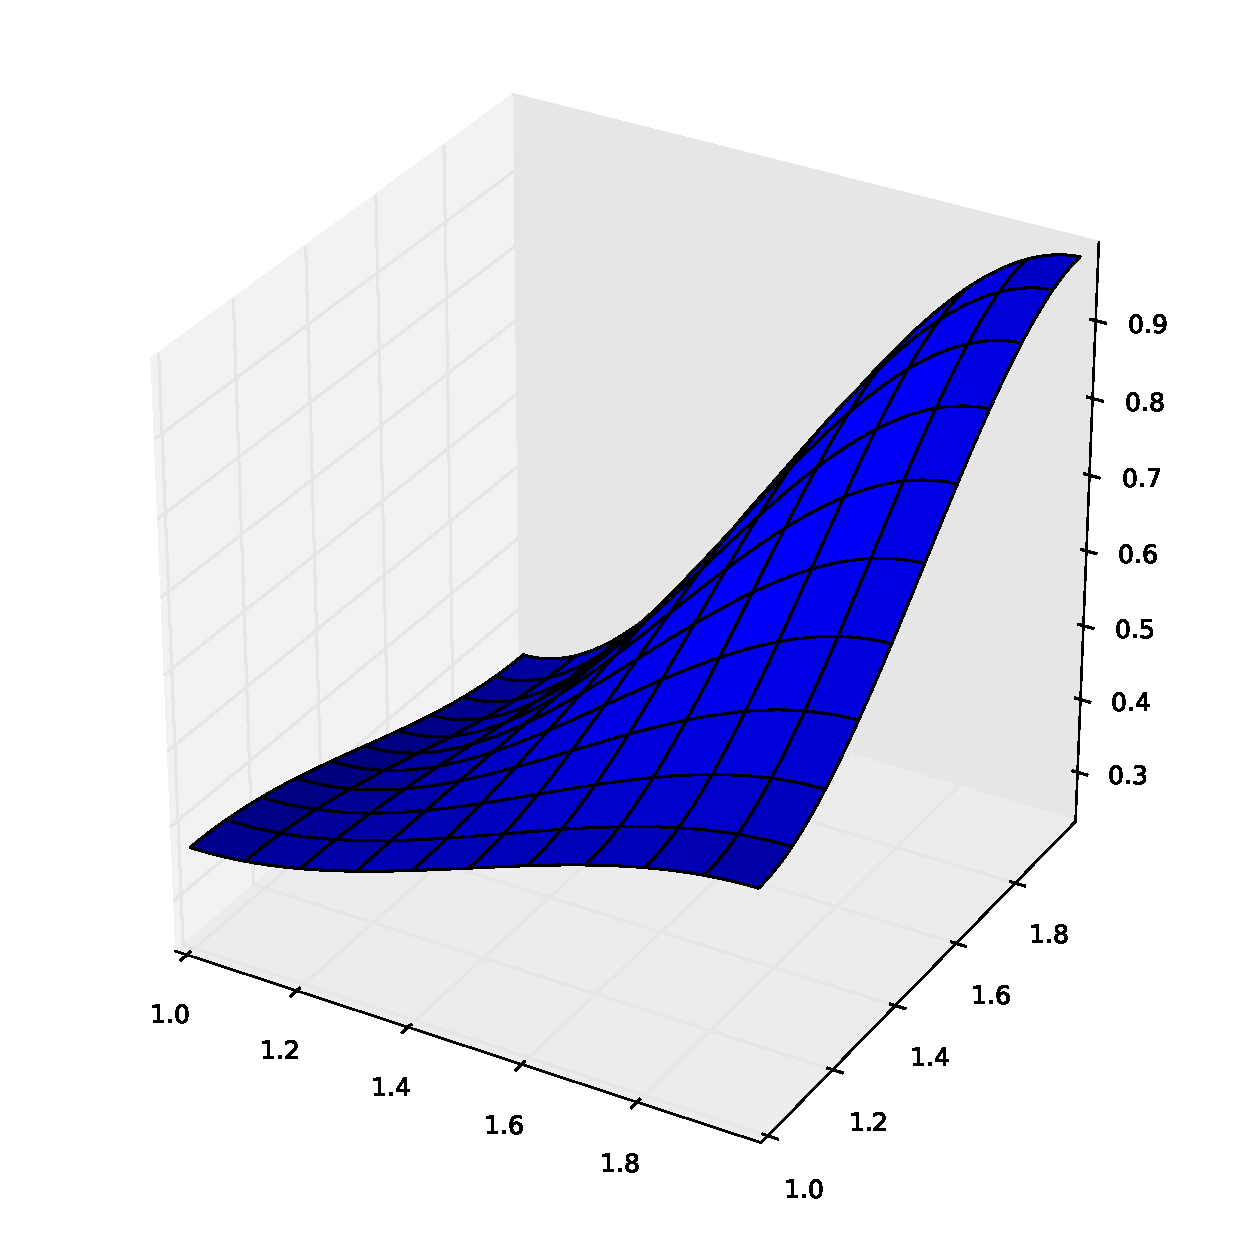
\includegraphics[width=\textwidth]{onesquaresurface.eps}
\end{columns}
\end{frame}




\sect{Smooth Noise in 2D}
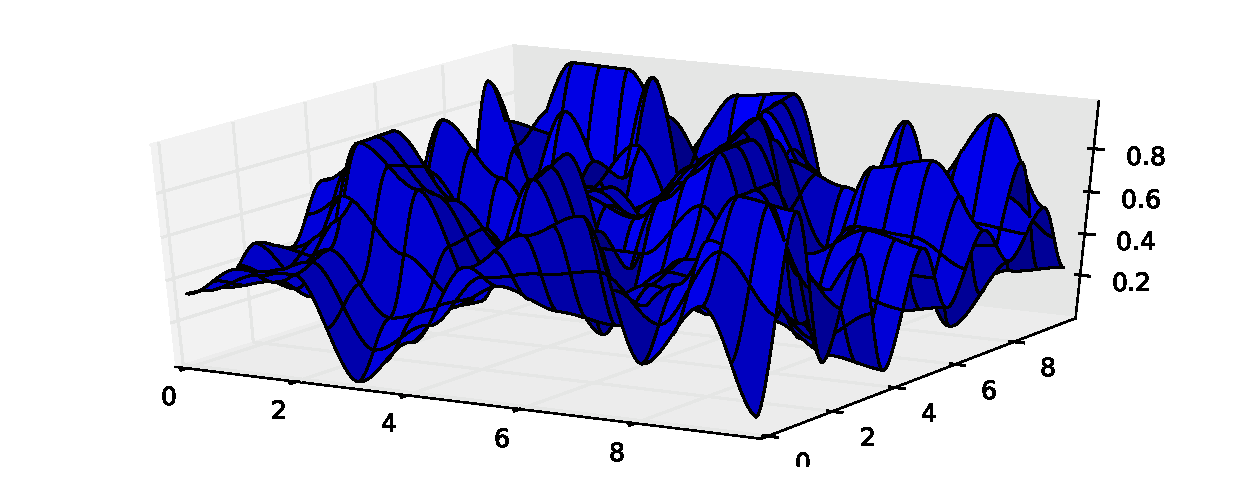
\includegraphics[width=\textwidth]{smoothnoisesurface.eps}
\begin{itemize}
\item Doing this over the whole lattice gives us smooth noise in 2D.
\end{itemize}
\end{frame}

\sect{Pink Noise in 2D}
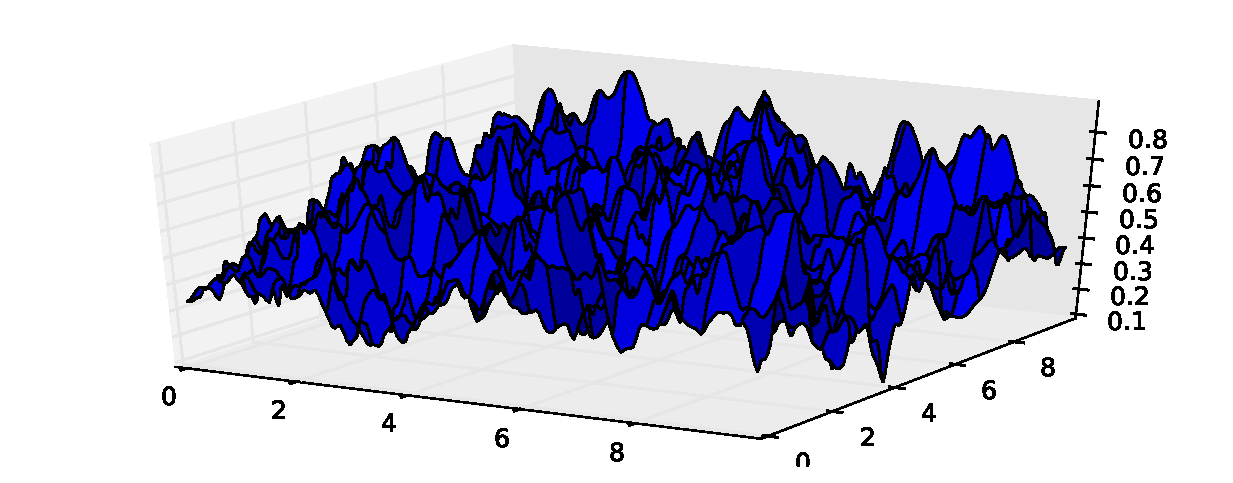
\includegraphics[width=\textwidth]{pinknoisesurface.eps}
\begin{itemize}
\item If we add up many smooth noises of shorter wavelength and
  smaller amplitude we end up with 2D pink noise.

\end{itemize}
\end{frame}

\sect{Pink Noise in 2D}
\begin{itemize}
\item Smooth noises at diminishing wavelengths:

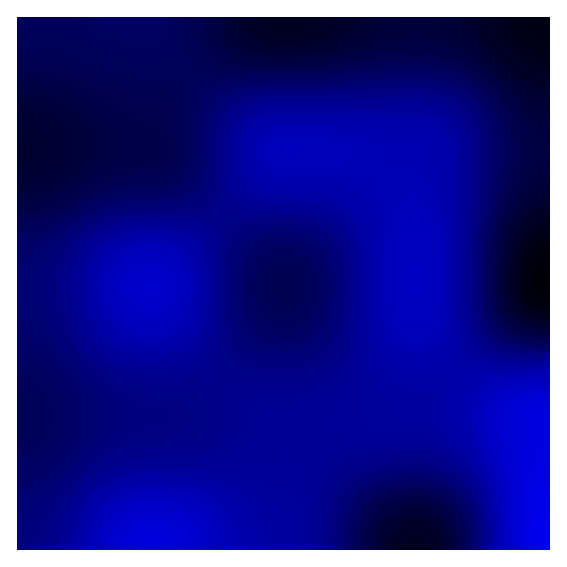
\includegraphics[width=.15\textwidth]{twoDone.eps}\hfill
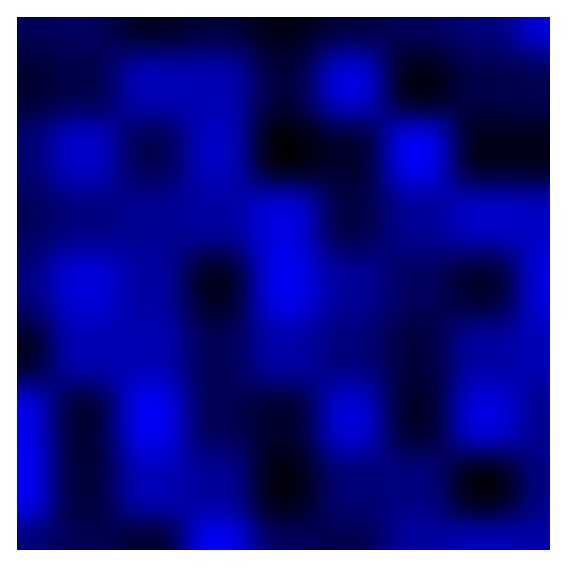
\includegraphics[width=.15\textwidth]{twoDtwo.eps}\hfill
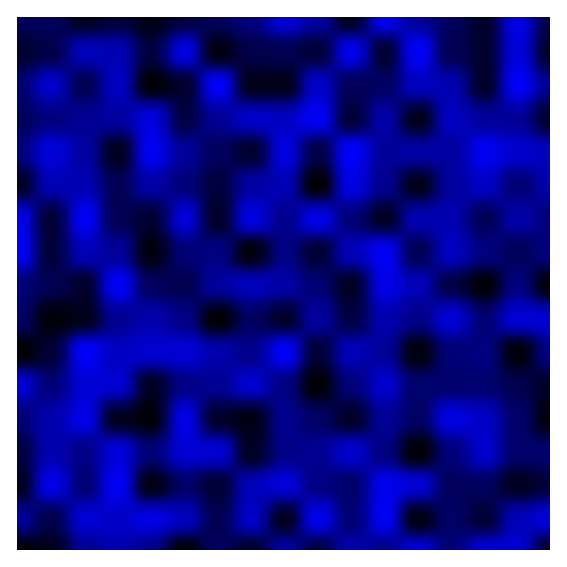
\includegraphics[width=.15\textwidth]{twoDthree.eps}\hfill
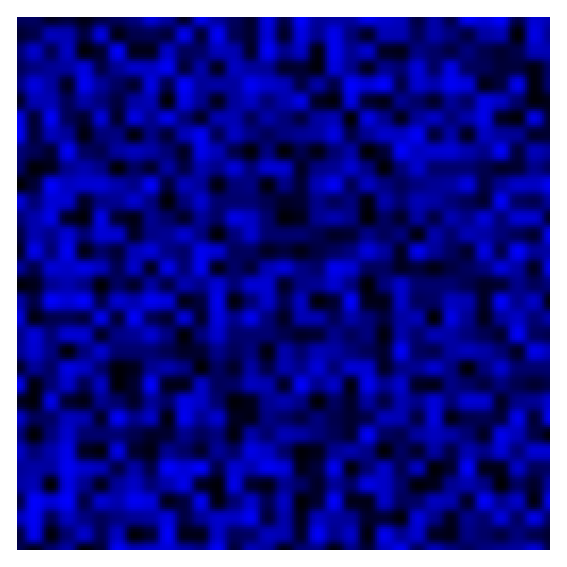
\includegraphics[width=.15\textwidth]{twoDfour.eps}\hfill
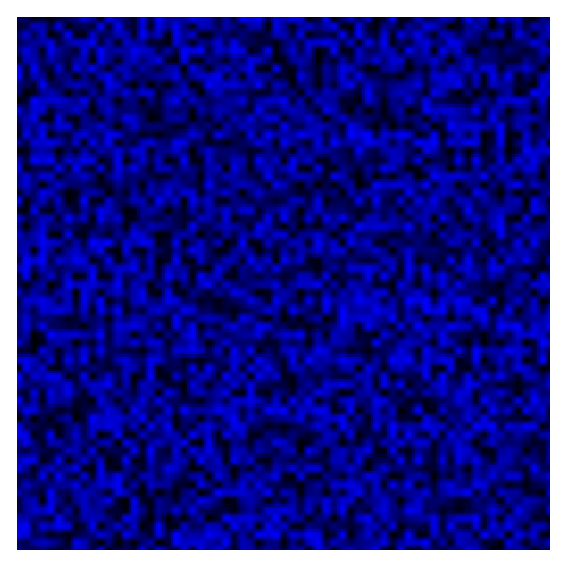
\includegraphics[width=.15\textwidth]{twoDfive.eps}\hfill
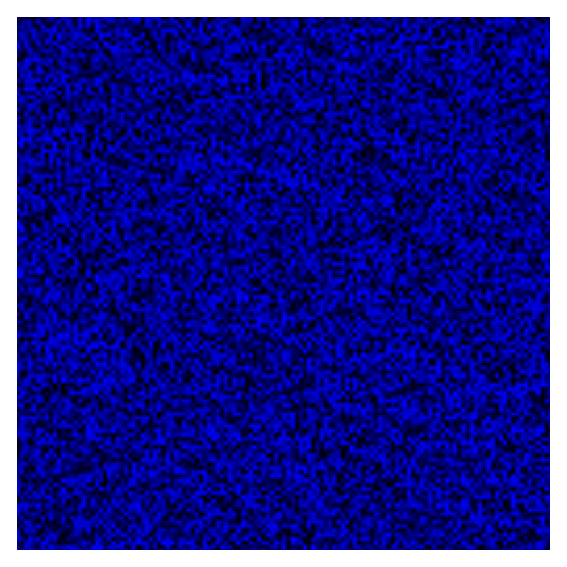
\includegraphics[width=.15\textwidth]{twoDsix.eps}

\item The pink noise sum of the above, amplitude diminishing with
  wavelength:

\centerline{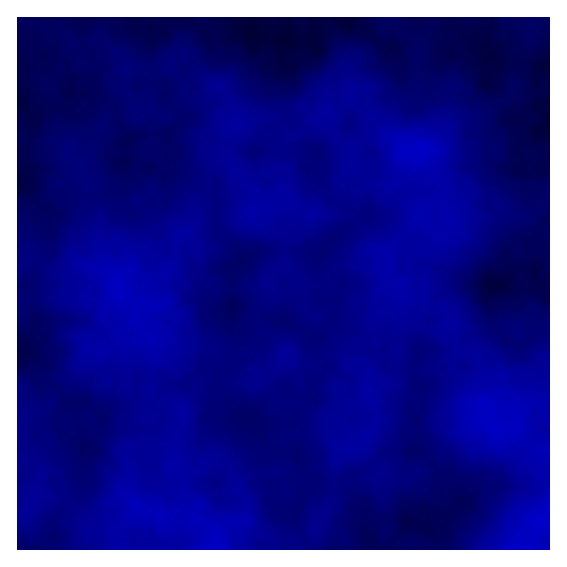
\includegraphics[width=.30\textwidth]{pinknoise.eps}}

\end{itemize}

\end{frame}

\sect{Colorizing noise for different effects}


\includegraphics[width=0.5\textwidth]{sky.eps}\hfill
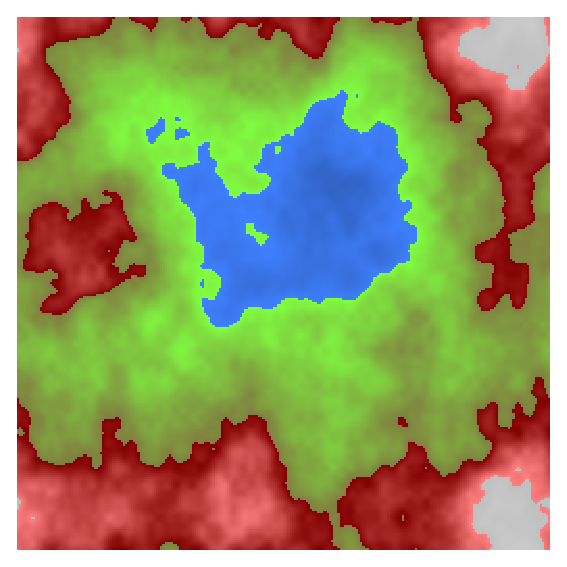
\includegraphics[width=0.5\textwidth]{terrain.eps}

Sky \hfill Terrain 

\end{frame}

\sect{Effects of starting wavelength and number of octaves}
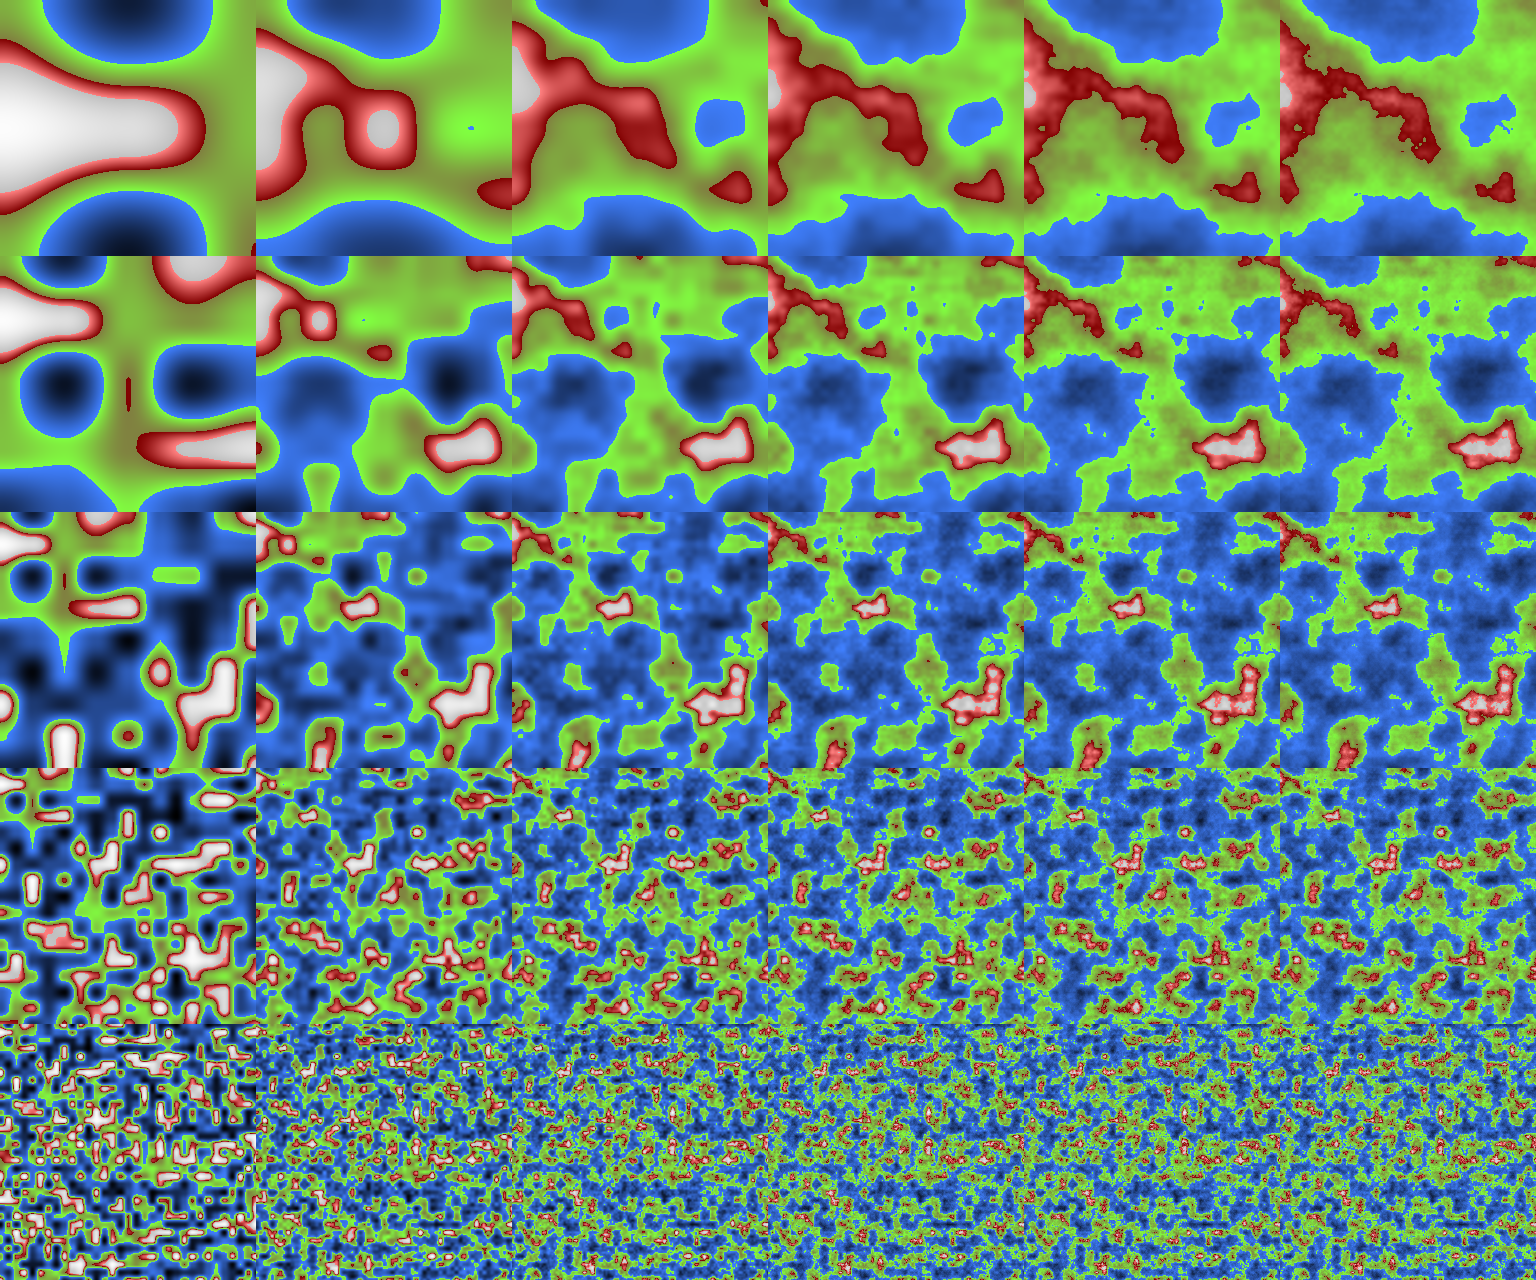
\includegraphics[width=\textwidth]{parameters.eps}
\end{frame}

\sect{Tilable noise}
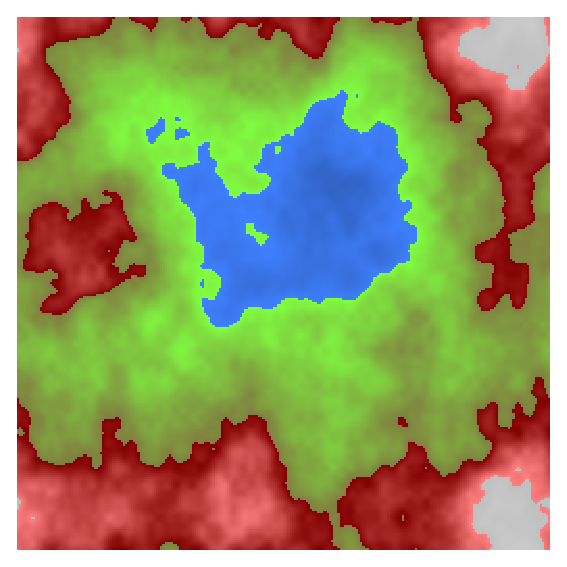
\includegraphics[width=0.4\textwidth]{terrain.eps}
\hfill
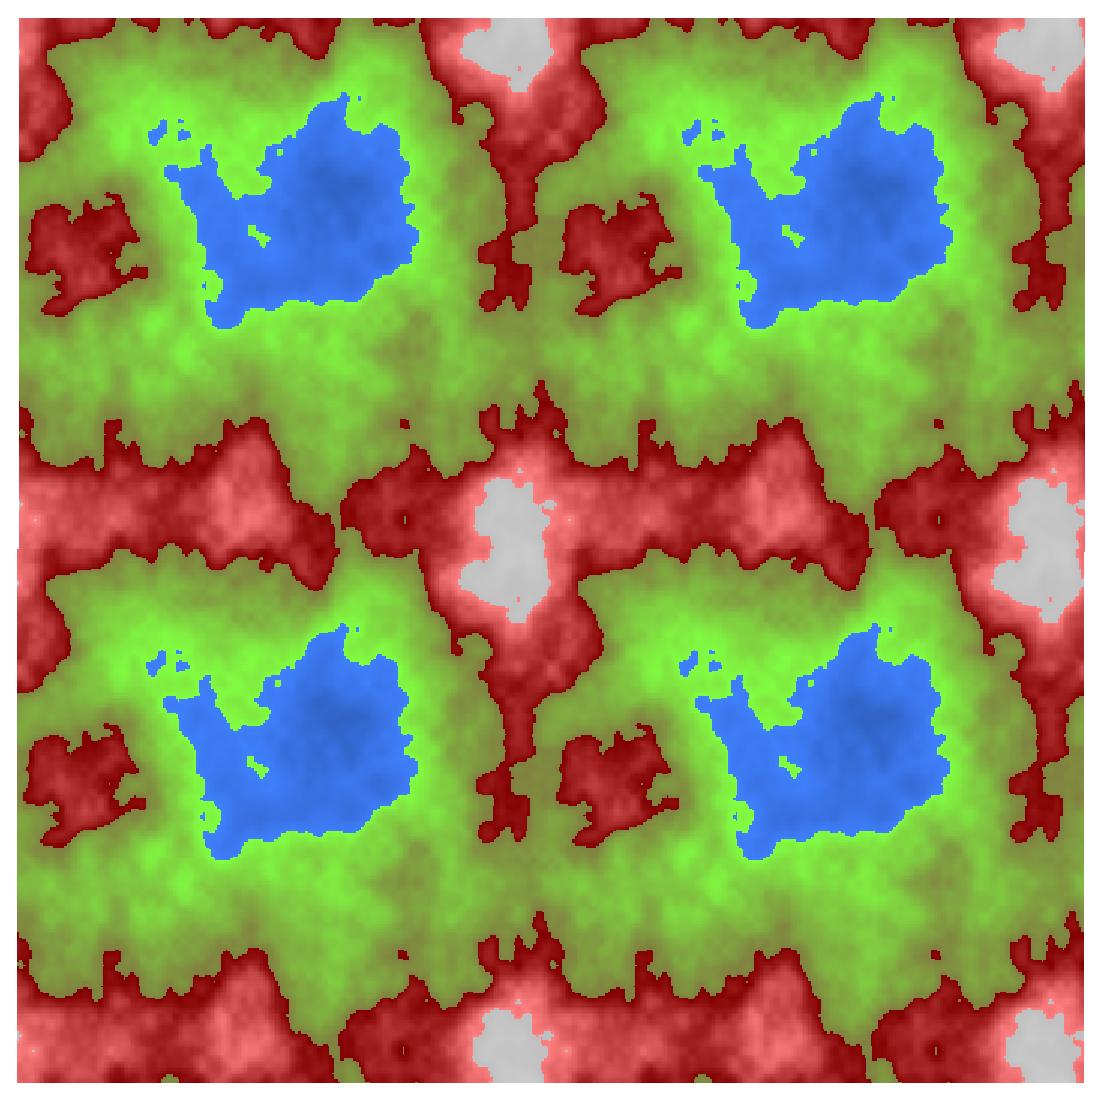
\includegraphics[width=0.5\textwidth]{tiledterrain.eps}
\begin{itemize}
\item How can we do this?
\end{itemize}
\end{frame}

\sect{Tilable noise}

\includegraphics[width=0.4\textwidth]{sky.eps}
\hfill
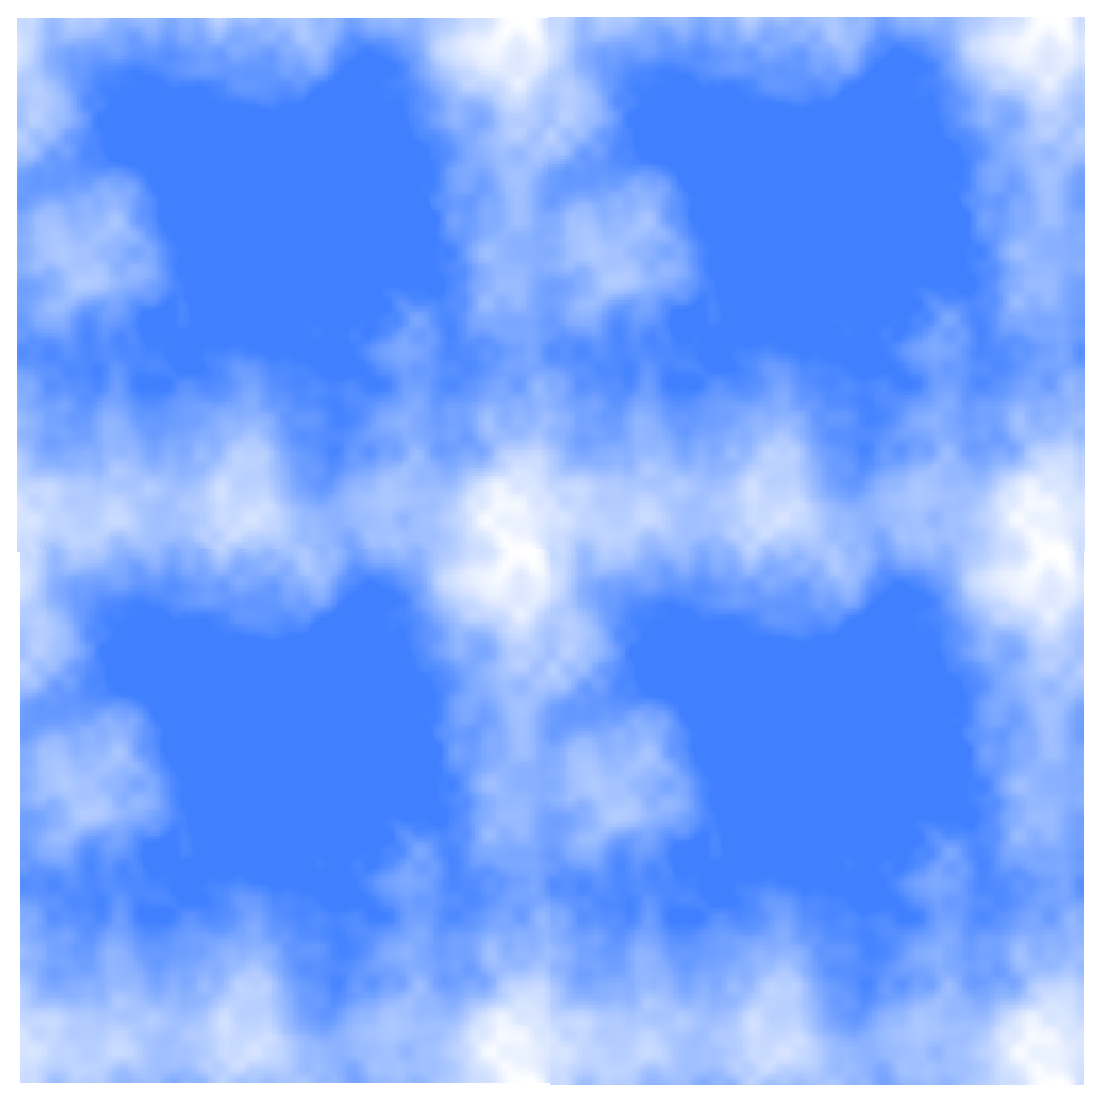
\includegraphics[width=0.5\textwidth]{tiledsky.eps}
\end{frame}

\sect{3D noise: solid textures and animations }
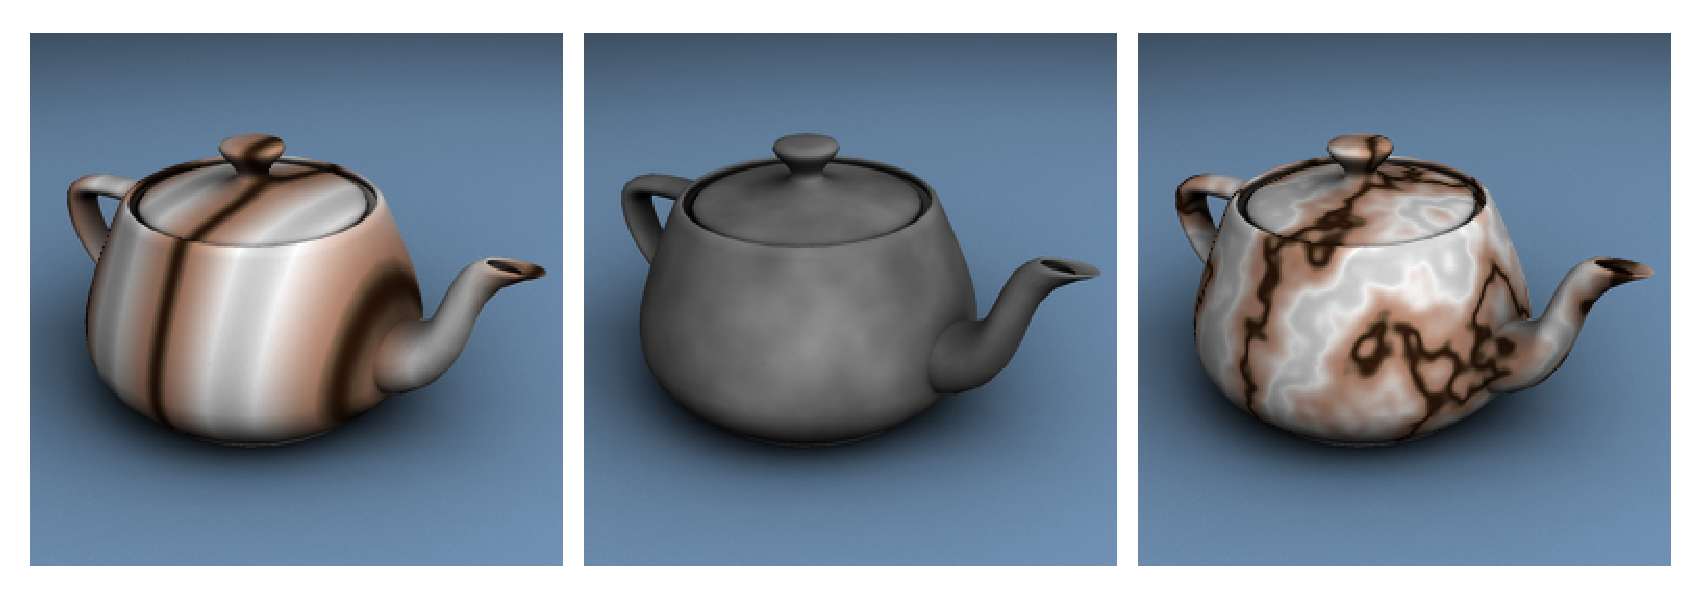
\includegraphics[width=\textwidth]{noise3d.eps}

\end{frame}

\sect{Online Resources}
{\bf Readings}
\begin{itemize}
\myref{http://www.noisemachine.com/talk1/}
\myref{http://freespace.virgin.net/hugo.elias/models/m_perlin.htm}
\myref{http://en.wikipedia.org/wiki/White_noise}
\myref{http://en.wikipedia.org/wiki/Pink_noise}
\myref{http://mrl.nyu.edu/~perlin/doc/oscar.html}
\myref{http://legakis.net/justin/MarbleApplet/}
\myref{http://www.planetside.co.uk/}
\end{itemize}
{\bf Grad students:}
\begin{itemize}
\myreft{http://webstaff.itn.liu.se/~stegu/simplexnoise/simplexnoise.pdf}
\end{itemize}

\end{frame}


\end{document}
